% Figura cuerpo B2: solo la expansión monetaria imprevista mueve la producción
\documentclass[tikz,border=3pt]{standalone}
\usepackage[T1]{fontenc}
\usepackage[utf8]{inputenc}
\usepackage{amsmath}
\usetikzlibrary{arrows.meta,calc,positioning}
\begin{document}
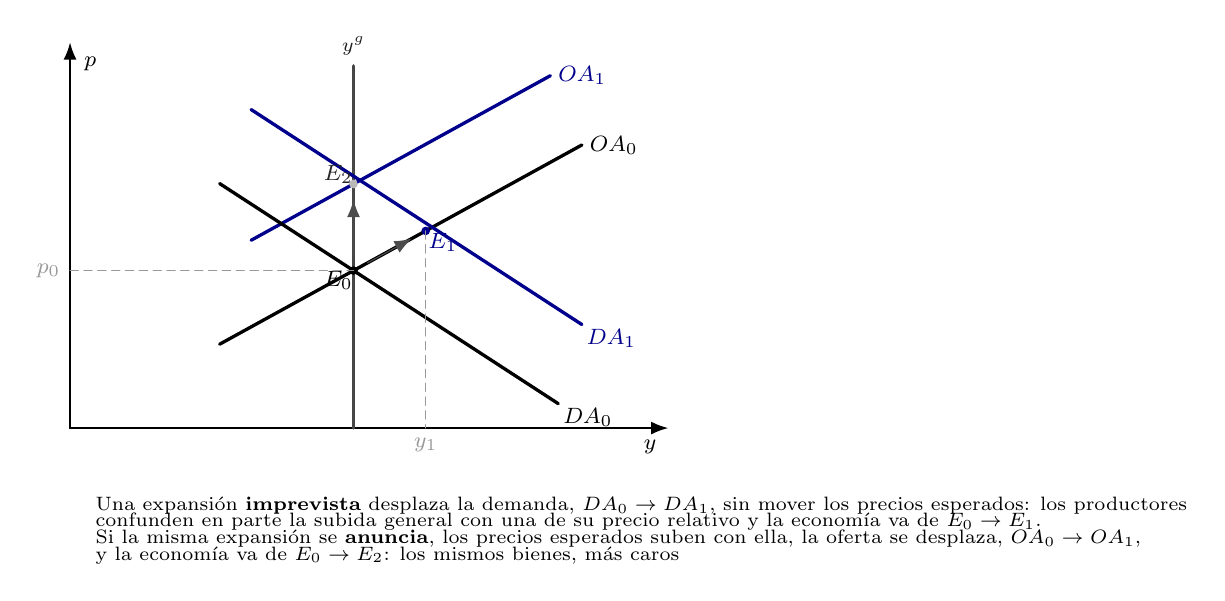
\begin{tikzpicture}[>={Latex[length=2.2mm]}, line cap=round, font=\footnotesize,
  eje/.style={->, thick},
  curva/.style={very thick},
  nueva/.style={very thick, blue!55!black},
  guia/.style={densely dashed, gray!80},
  pto/.style={circle, fill=black, inner sep=1.1pt}]
  \draw[eje] (0,0) -- (7.6,0) node[below left=1pt]{$y$};
  \draw[eje] (0,0) -- (0,4.9) node[below right=2pt]{$p$};
  % Tendencia
  \draw[curva, gray!55!black] (3.6,0) -- (3.6,4.6) node[above, font=\scriptsize, text=gray!25!black]{$y^{g}$};
  % Oferta de LUCAS
  \draw[curva] (1.9,1.065) -- (6.5,3.595) node[right=-1pt]{$OA_0$};
  \draw[nueva] (2.3,2.385) -- (6.1,4.475) node[right=-1pt]{$OA_1$};
  % Demanda
  \draw[curva] (1.9,3.105) -- (6.2,0.31) node[below right=-3pt]{$DA_0$};
  \draw[nueva] (2.3,4.045) -- (6.5,1.315) node[below right=-3pt]{$DA_1$};
  % Equilibrios
  \node[pto] (E0) at (3.6,2.0) {};
  \node[below left=-3pt of E0, inner sep=1pt] {$E_0$};
  \node[pto, fill=blue!55!black] (E1) at (4.517,2.504) {};
  \node[below right=-2pt of E1, inner sep=1pt, blue!55!black] {$E_1$};
  \node[pto, fill=gray!55] (E2) at (3.6,3.1) {};
  \node[above left=-3pt of E2, inner sep=1pt, gray!30!black] {$E_2$};
  \draw[guia] (4.517,2.504) -- (4.517,0) node[below]{$y_1$};
  \draw[guia] (0,2.0) node[left]{$p_0$} -- (3.6,2.0);
  \draw[->, gray!60!black, shorten >=4pt, shorten <=4pt] (E0) -- (E1);
  \draw[->, gray!60!black, shorten >=4pt, shorten <=4pt] (E0) -- (E2);
  \node[align=left, anchor=north west, font=\scriptsize] at (0.2,-0.75)
    {Una expansión \textbf{imprevista} desplaza la demanda, $DA_0\to DA_1$, sin mover los precios esperados: los productores\\[-2pt]confunden en parte la subida general con una de su precio relativo y la economía va de $E_0\to E_1$.\\[-2pt]Si la misma expansión se \textbf{anuncia}, los precios esperados suben con ella, la oferta se desplaza, $OA_0\to OA_1$,\\[-2pt]y la economía va de $E_0\to E_2$: los mismos bienes, más caros};
\end{tikzpicture}
\end{document}
